\section{Travail r\'{e}alis\'{e}}

Tout au long de cette mission, ou plut\^{o}t ces missions (un test achev\'{e} laisse toujours la place \`{a} un autre), j'ai travaill\'{e} \`{a} impl\'{e}menter des tests en \gls{Java} permettant de valider automatiquement le comportement de WebI au niveau SDK.

L'objectif principal de cette mission \'{e}tait d'\^{e}tre, \`{a} terme, capable d'impl\'{e}menter seul et dans les plus brefs d\'{e}lais un test automatique. La grande difficult\'{e} de d\'{e}but de cette mission a \'{e}t\'{e} de comprendre, d'une part, la logique du \gls{Framework}\index{Framework} de test, et d'autre part les diff\'{e}rentes choses que celui-ci me permettait de faire.\\

Les concepts \`{a} assimiler \'{e}taient nombreux et j'ai pass\'{e} beaucoup de temps \`{a} essayer de comprendre le \gls{Framework} sur lequel repose l'impl\'{e}mentation des tests. Les probl\`{e}mes majeurs que j'ai rencontr\'{e}s au d\'{e}but sont les diff\'{e}rents points suivants :
\begin{itemize}
	\item Comment int\'{e}grer un test \`{a} l'ensemble des tests ex\'{e}cut\'{e}s?
  \item Quel type de test mettre en place, statique ou dynamique?
	\item Comment initialiser un test?
	\item Comment g\'{e}rer les sources de telle ou telle version du logiciel pour impl\'{e}menter un test automatique?
	\item O\`{u} trouver les fichiers de r\'{e}f\'{e}rences n\'{e}cessaires?
\end{itemize}

J'ai \'{e}clairci tous ces points au fur et \`{a} mesure de mes missions et de mes exp\'{e}rimentations. Certains sont tr\`{e}s simples \`{a} assimiler mais d'autres m'ont pos\'{e}s beaucoup de probl\`{e}mes. Je d\'{e}taille dans les parties suivantes comment est-ce que j'ai \'{e}t\'{e} confront\'{e} \`{a} ces diff\'{e}rents probl\`{e}mes et la mani\`{e}re dont je m'y suis pris pour les r\'{e}soudre. Dans la partie qui suit je pr\'{e}senterai les diff\'{e}rents probl\`{e}mes que j'ai rencontr\'{e} et la mani\`{e}re dont je m'y suis pris pour les r\'{e}soudre. Dans le souci de rester clair dans mes explications je ne m'\'{e}parpillerai pas sur tous les tests que j'ai impl\'{e}ment\'{e} qui m'ont mis face \`{a} tel ou tel probl\`{e}me. Je partirai plut\^{o}t d'un cas simple de test automatique en consid\'{e}rant que tous ces probl\`{e}mes se sont succ\'{e}d\'{e}s dans le cadre du m\^{e}me test.\\


\subsection{Les recherches relatives aux tests automatiques dans le cadre du \gls{Framework} utilis\'{e}}


Ne connaissant rien ni de Web Intelligence ni du \gls{Framework} de test, je me suis d'abord pench\'{e} la mani\`{e}re d'utiliser ce \gls{Framework} pour impl\'{e}menter un code simple manipulant un document Web Inteliigence.\\

Pour se faire, j'ai choisi une fonctionnalit\'{e} tr\`{e}s simple, le d\'{e}placement d'une cellule dans un tableau, me basant sur un document de test mis \`{a} ma disposition (illustration de ce document figure \pageref{figure:docsample}).\\

\begin{figure}[!h]
  \centering
      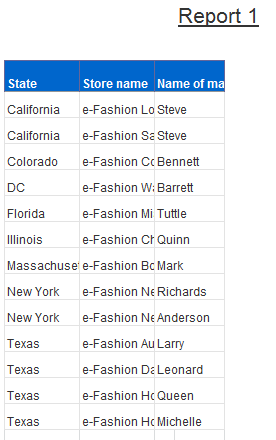
\includegraphics{images/docsample.png}
  \caption{Document sur lequel j'ai bas\'{e} mes premi\`{e}re exp\'{e}rimentations}
	\label{figure:docsample}
\end{figure}
 
Partant de ce document, comment devais-je m'y prendre pour automatiser une action sur celui-ci? Pour se faire il me fallait me baser sur une impl\'{e}mentation de test automatique d\'{e}j\`{a} exitante. J'ai donc chercher un code dont la structure me permettait de manipuler un document Web Intelligence d\'{e}j\`{a} existant. Il en existe beaucoup de types diff\'{e}rents mais j'ai rapidement trouv\'{e} l'exemple d'un test qui se basait sur un document Web Intelligence. J'ai donc cr\'{e}\'{e} une nouvelle \gls{Classe} pour mon test et ai coll\'{e} le code \'{e}pur\'{e} \`{a} l'int\'{e}rieur, j'avais donc une \gls{Classe} \gls{Java} me permettant d'effectuer un test sur mon document. Mais \`{a} cette \'{e}tape j'ai rencontr\'{e} un certain nombre de probl\`{e}mes m'emp\^{e}chant de tester mon code qui ne compilait pas.\\
J'ai pass\'{e} beaucoup de temps \`{a} chercher les solutions dans les messages d'erreurs que je re\c{c}evais en masse.\\

J'avais pris le soin de coller mon document Web Intelligence pr\'{e}cis\'{e}ment dans le dossier qu'il fallait mais pourtant, les messages d'erreur me disait que le document \'{e}tait introuvable. En investiguant tous les documents rentrant en jeu dans l'ex\'{e}cution du test et en r\'{e}fl\'{e}chissant \`{a} la signification de chacune des variables, je me suis rendu compte que je n'avais pas modifi\'{e} le \textquote{script ID} du fichier script.xml. Celui-ci permet d'identifier un plan de test, qui lui-m\^{e}me identifie une ou plusieurs \gls{Classe}s de test. Une fois la modification effectu\'{e}e, en prenant soin de correctement renseigner le nom de mon test, je suis tomb\'{e} une fois de plus sur une erreur similaire : le document demeure introuvable. Le plan de test \'{e}tant ex\'{e}cut\'{e}, cette fois-ci, l'erreur ne pouvait se trouver que dans ma \gls{Classe} de test. J'ai rapidement identifi\'{e} le probl\`{e}me puisque c'est dans cette m\^{e}me \gls{Classe} que le chemin d'acc\`{e}s \`{a} mon fichier est renseign\'{e}. Les r\'{e}pertoires \'{e}tant nomm\'{e}s diff\'{e}remment en fonction de la suite de test \`{a} laquelle ils appartiennent, et, le test que je voulais ex\'{e}cuter ne faisant pas partie de la m\^{e}me suite, lors de l'ex\'{e}cution \gls{Java} n'allais pas chercher mon document dans le bon r\'{e}pertoire. J'ai donc corrig\'{e} cette erreur et ai renseign\'{e} la bonne valeur.\\
En ex\'{e}cutant de nouveau, je constate qu'il n'y a plus de probl\`{e}mes d'acc\`{e}s \`{a} un fichier. Cette fois-ci les messages d'erreur m'annoncent qu'il est impossible d'acc\'{e}der au \gls{CMS}. Je me dirige donc vers le \gls{CMS} en question pour r\'{e}cup\'{e}rer son adresse puis vers le fichier parameters.xml dans lequel l'url du \gls{CMS} est renseign\'{e}e, effectivement ce n'\'{e}tait pas la m\^{e}me, mais d'autre part en essayant d'acc\'{e}der au \gls{CMS} dont il \'{e}tait question je constatais que celui-ci n'existait plus, je ne pouvais pas y acc\'{e}der. J'ai donc corrig\'{e} l'adresse du \gls{CMS} sur lequel je voulais faire mon test.\\
En ex\'{e}cutant une fois de plus j'ai \'{e}t\'{e} ravi de voir que mon test compilais, celui-ci ne faisait encore rien mais je pouvais alors commencer \`{a} manipuler mon document Web Intelligence en impl\'{e}mentant le code de mon test automatique.\\

La question qui se posa alors \'{e}tait de savoir comment y acc\'{e}der et de quelle mani\`{e}re m'y prendre pour le modifier.\\
En parcourant les tests automatiques existants et en cherchant les informations qui me manquaient, j'ai constat\'{e} avec surprise que nul part dans le code il n'y avait de commentaires pour expliquer la d\'{e}marche utilis\'{e}e ou la logique appliqu\'{e}e. Ce qui m'a troubl\'{e}, puisque l'on m'avais toujours enseign\'{e} que les commentaires sont essentiels dans toute impl\'{e}mentation. J'ai \'{e}videmment pos\'{e} la question pour en connaitre la raison. Les \'{e}quipes de d\'{e}veloppement et de test de Web Intelligence travaillant en suivant la m\'{e}thode agile, celles-ci sont cens\'{e}es \'{e}crire des codes clairs au point que le code lui-m\^{e}me suffit \`{a} sa compr\'{e}hension. Les quelques rares commentaires servant \`{a} expliquer le fonctionnement g\'{e}n\'{e}ral d'une grande portion de code. Je comprenais ce principe mais j'\'{e}tais d\'{e}rang\'{e} par le fait que chacun des objets utilis\'{e}s dans le code m'\'{e}taient inconnus, ce qui augmentait beaucoup le temps qu'il me fallait pour comprendre une certaine impl\'{e}mentation.\\ 

En cherchant parmi les tests automatiques existants j'ai trouv\'{e} le code qui me permettrait de r\'{e}cup\'{e}rer mon document :
\begin{lstlisting}
IRSReport monRapport = docCalc.getReportAurora(0);
\end{lstlisting}

L'objet \textquote{docCalc} appartenant \`{a} la super \gls{Classe} de ma \gls{Classe} de test, contient un grand nombre de m\'{e}thodes permettant de manipuler un document Web Intelligence. L'argument \textquote{0} que je passe \`{a} la m\'{e}thode me permet de r\'{e}cup\'{e}rer le premier rapport que contient mon document. Pour compl\'{e}ter ce code ci-dessus et le faire ressembler \`{a} test il faut marquer le d\'{e}but et la fin du test. Le code compl\'{e}t\'{e} \'{e}tant le suivant :


\begin{lstlisting}
IRSReport reportAurora = docCalc.getReportAurora(0);
startTestcaseStep("monTest");
stopTestcaseStepWithAction();
\end{lstlisting}
 
En observant les logs de l'ex\'{e}cution de ce test, on remaque que la premi\`{e}re m\'{e}thode \textquote{startTestcaseStep("");} permet de marquer le d\'{e}but des tests, celle-ci ne fait rien d'autre que d'ajouter un log. Ensuite, \textquote{stopTestcaseStepWithAction();} marque non seulement la fin du test dans les logs mais aussi ex\'{e}cute une s\'{e}rie d'actions qui sont d\'{e}critent dans les logs. Il est int\'{e}ressant de les noter ici car ces actions peuvent nous \^{e}tre tr\`{e}s utiles.\\
L'\'{e}tude des ces logs m'a \'{e}t\'{e} d'une grande aide car ceux-ci d\'{e}crivent pr\'{e}cis\'{e}ment l'ex\'{e}cution du test.\\




\subsubsection{Recherche effectu\'{e}es pour conna\^{i}tre les diff\'{e}rentes actions de l'ex\'{e}cution d'un test}
Les logs sont nombreux et j'ai pass\'{e} beaucoup de temps \`{a} les analyser. J'ai pu en conclure les trois \'{e}tapes essentielles, et \'{e}videntes, de l'ex\'{e}cution d'un test : l'avant test, le pendant et l'apr\`{e}s. Un exemple d'une de ces sorties consoles que j'ai ainsi \'{e}tudi\'{e} est disponible annexe \ref{annexe:sortieConsole} page \pageref{annexe:sortieConsole} dans laquelle j'ai distingu\'{e} les diff\'{e}rentes parties depuis lesquelles les logs \'{e}taient g\'{e}n\'{e}r\'{e}s.\\
Pour faire ces obsvervations j'ai simplement ajout\'{e} des logs au moments cl\'{e}s de l'ex\'{e}cution : au d\'{e}but et \`{a} la fin du constructeur et de mon test (en distinguant la m\'{e}thode de test et l'impl\'{e}mentation du test). Cela m'a permis d'observer et ainsi de comprendre les diff\'{e}rentes \'{e}tapes du test tels qu'ils \'{e}taient dans le \gls{Framework} que j'utilisais. Les tests que j'impl\'{e}mentais \'{e}taient ex\'{e}cut\'{e}s dans un cycle propre au \gls{Framework}, cycle qui m'\'{e}tait inconnu et sans documentation. De cette mani\`{e}re j'ai pu, d'une part, observer dans quelle ex\'{e}cution s'inscrivait mon test, d'autre part, \'{e}tudier l'ex\'{e}cution de mon test lui-m\^{e}me et comprendre l'utilit\'{e} de certaines fonctions. Ci-dessous la liste d\'{e}scriptive de ce que j'ai pu d\'{e}duire de cette \'{e}tude (la m\'{e}thode \textquote{run()} dont je parle et la m\'{e}thode contenant l'impl\'{e}mentation de mon test automatique) :

\begin{enumerate}
	\item Avant la m\'{e}thode \textquote{run()}
	\begin{itemize}
		\item Avant toute chose, ce sont les informations contenues dans le fichier parameters.xml qui sont r\'{e}cup\'{e}r\'{e}es, autrement dit, le \gls{CMS} sur lequel le test devra \^{e}tre effectu\'{e}
		\item V\'{e}rifie l'existence du dossier contenant les ressources utilis\'{e}s dans le cadre de tout test
		\item Cr\'{e}ation du fichier dans lequel seront enregistr\'{e}s les logs 
		\item Connexion au serveur (CSM)
		\item Recherche le dossier FavoritesFolder sur le \gls{CMS}
		\item Supprime, en local, les dossier o\`{u} sont enregistr\'{e}s les r\'{e}sultats (\textbackslash res\textbackslash  et \textbackslash ref\textbackslash )
		
	\end{itemize}
	\item Pendant la m\'{e}thode \textquote{run()} et avant la m\'{e}thode \textquote{stopTestcaseStepWithAction();}
	\begin{itemize}
		\item Recherche de l'univers mentionn\'{e} dans l'impl\'{e}mentation du test automatique
		\item Cr\'{e}ation d'un nouveau document sur les \gls{CMS}, celui-ci est suivi du nom que j'ai donn\'{e} \`{a} l'ex\'{e}cution de mon test (\textquote{startTestcaseStep("monTest");}) de telle sorte que je vais retrouv\'{e} sur le \gls{CMS} le document que j'avais en local.
	\end{itemize}
	\item Pendant la m\'{e}thode \textquote{stopTestcaseStepWithAction();} (cette m\'{e}thode \'{e}tant comprise dans la m\'{e}thode \textquote{run()})
	\begin{itemize}
		\item Cr\'{e}ation du dossier o\`{u} les r\'{e}sultats seront enregistr\'{e}s
		\item Recherche le dossier \textquote{Personnal Documents} sur le \gls{CMS}
		\item Recherche sur le \gls{CMS} du document concern\'{e} par mon test (ce document se retrouve en deux endroits et dans deux \'{e}tats diff\'{e}rents, sur le \gls{CMS} et en local, avant test et apr\`{e}s test)
		\item Sauvegarde du document en local
		
	\end{itemize}
	\item Apr\`{e}s la m\'{e}thode \textquote{run()}
	\begin{itemize}
		\item Sauvegarde du document dans le personal folder du \gls{CMS}
		\item Copie la r\'{e}f\'{e}rence du cube (r\'{e}f\'{e}rence que j'ai moi-m\^{e}me d\'{e}pos\'{e}) vers le dossier \textbackslash ref\textbackslash
		\item Cr\'{e}e le dossier qui recevra les r\'{e}f\'{e}rences
		\item Compare le document cr\'{e}\'{e} avec la r\'{e}f\'{e}rence
	\end{itemize}
\end{enumerate}

Durant cette partie de mon travail, o\`{u} l'investigation c'est \'{e}tal\'{e}e sur plusieurs semaines et portant sur plusieurs tests \`{a} impl\'{e}menter, j'ai d\'{e}couvert \'{e}norm\'{e}ment de choses aussi bien en \gls{Java} que sur l'utilisation du \gls{Framework} de test. J'ai pu mettre au point des m\'{e}thodes de r\'{e}solution de mes probl\`{e}mes et ai pu d\'{e}couvrir la majeure partie des objets utilis\'{e}s lors de l'impl\'{e}mentation des tests automatiques de Web Intelligence.


\subsubsection{Modification d'un document Web Intelligence gr\^{a}ce au \gls{Framework}}

Ayant maintenant \'{e}tudi\'{e} toute l'ex\'{e}cution du test, je suis plus \`{a} m\^{e}me de situer le test automatique dans sa globalit\'{e}.\\
La question qui se pose maintenant est de savoir quoi mettre dans le test, avant de pouvoir se poser la vraie question : \textquote{Comment tester automatiquement une fonctionnalit\'{e}?}. Au d\'{e}but, je consid\'{e}rai que toute modification applicable depuis l'interface graphique pouvait \^{e}tre reproduite depuis le test. J'avais tord. Mes tests automatiques \'{e}tant des tests au niveau SDK, les fonctionnalit\'{e}s auxquelles j'avais acc\`{e}s et que je pouvais tester \'{e}taient donc limit\'{e}es \`{a} celui-ci.\\

Pour en revenir \`{a} l'impl\'{e}mentation de mon test de base, devant d\'{e}placer une cellule, la mani\`{e}re la plus simlple \'{e}tait de trouver quelque part dans les tests existants comment cette fonctionnalit\'{e} \'{e}tait utilis\'{e}e. Je n'ai pas trouv\'{e} d'exemple me permettant d'appliquer rapidement ce changement \`{a} mon document mais j'ai trouv\'{e} des pistes qui para\^{i}ssaient prometteuses. La recherche du mot \textquote{drop} dans le \gls{Framework} m'a retourn\'{e} beaucoup de r\'{e}sultats dont un qui a retenu mon attention, il existe un objet \textquote{DropHelperImpl}. On en d\'{e}duit assez facilement, \`{a} partir de son nom, que celui \`{a} quelque chose \`{a} voir avec le d\'{e}placement d'une cellule. Il me fallait trouver un exemple d'utilisation de cet objet pour faciliter mon travail, fort heureusement il existe une fonctionnalit\'{e} d'\gls{Eclipse} que je ne connaissais pas avant (et que, depuis lors, je me suis mis \`{a} utiliser syst\'{e}matiquement) : \textquote{get call heirarchy}, me permettant d'avoir le d\'{e}tail de tous les emplacements o\`{u} cette \gls{Classe} est instanci\'{e}e. De cette mani\`{e}re j'ai rapidement trouv\'{e} des exemple de codes me permettant d'en d\'{e}duire les quelques informations qui m'\'{e}taient n\'{e}cessaires.\\

J'ai comprise que je ne pouvais pas faire ce que je voulais directement, il me fallait pr\'{e}parer le terrain et r\'{e}cup\'{e}rer tous les objets qui entraient en jeu dans le d\'{e}placement de la cellule.\\

Il fallait d'abord r\'{e}cup\'{e}rer, \'{e}videmment, le corps de mon document, cela se fait simplement gr\^{a}ce \`{a} l'une des M\'{e}thodes propres au rapport :
\begin{lstlisting}
reportAurora.getPageZone(PageZoneType.BODY);
\end{lstlisting}
L'\'{e}tape suivante \'{e}tait de r\'{e}cup\'{e}rer le tableau contenu dans le corps du document, le probl\`{e}me \'{e}tant que pour se faire il faut appeler l'objet par son nom. Comment savoir comment ce tableau a \'{e}t\'{e} appel\'{e}? Car je pouvais acc\'{e}der \`{a} mon document depuis Web Intelligence mais, depuis l'interface, je n'avais aucun moyen de savoir ce qui se passait derri\`{e}re, c\^{o}t\'{e} logiciel.\\
La m\'{e}thode que j'ai utilis\'{e} \`{a} ce moment l\`{a} et que j'ai toujours continu\'{e} \`{a} utiliser \'{e}tait de parcourir l'ensemble des \'{e}l\'{e}ments contenu dans le corps du rapport et d'en afficher les propri\'{e}t\'{e}s. Cela me permettais, non seulement, d'obtenir son nom, son identifiant et tout ses param\`{e}tres, mais aussi, d'obtenir son type. Au fur est \`{a} mesure du temps et que j'impl\'{e}mentais des tests j'ai d\'{e}couvert beaucoup de types diff\'{e}rents, leurs imbriquations, utilit\'{e}s et correspondances avec les \'{e}l\'{e}ments graphiques du document Web Intelligence.\\
Gr\^{a}ce \`{a} cette m\'{e}thode, j'ai pu d\'{e}terminer le nom de ce que je cherchais.\\
Ensuite, de cette table il me fallait r\'{e}cup\'{e}rer les colonnes, pour pouvoir les manipuler. Dans les diff\'{e}rents tests que j'avais pu \'{e}tudier auparavant, j'avais remarqu\'{e} l'utilisation d'une M\'{e}thode g\'{e}n\'{e}rique permettant de r\'{e}cup\'{e}rer une cellule d'un tableau. J'ai utilis\'{e} cette M\'{e}thode de la m\^{e}me mani\`{e}re que celle utilis\'{e}e dans les tests existants. \\
Alors j'ai pu impl\'{e}menter le code suivant qui me permettait de d\'{e}placer une colonne :


\begin{lstlisting}
IRSPageZone pageZone = reportAurora.getPageZone(PageZoneType.BODY);
IRSReportElement findReportElement = docCalc.findReportElement(pageZone.getChildren(), "Block 1");
IRSDynamicBlock table = (IRSDynamicBlock) findReportElement;
IRSCell cell1 = docCalc.getCellFromTable("State",(IRSTable) table);
IRSCell cell2 = docCalc.getCellFromTable("Store name ",(IRSTable) table);
IRSCell cell3 = docCalc.getCellFromTable("Name of manager ",(IRSTable) table);

DropHelperImpl dropHelp = new DropHelperImpl();
List<IRSCell> cells = new ArrayList<IRSCell>();
cells.add(cell1);
cells.add(cell2);
dropHelp.dropCells(cells, cell3, CellZone.RIGHT);
docCalc.applyFormat();
\end{lstlisting}

Au premier abord, l'utilisation de la \gls{Methode} \textquote{dropCells()} n'est pas instinctive, et j'ai fais plusieurs essais avant de comprendre son fonctionnement. Cette M\'{e}thode prends trois param\`{e}tres : un tableau de cellules, une cellule et une position. Le changement appliqu\'{e} par cette M\'{e}thode est que le contenu du tableau de cellule est d\'{e}plac\'{e} comme d\'{e}sir\'{e}, ici, \`{a} droite de la cellule sp\'{e}cifi\'{e}e.\\
La modification appliqu\'{e}e par ce code est illustr\'{e}e figure \ref{figure:dropcells}.\\

\begin{figure}[!h]
  \centering
      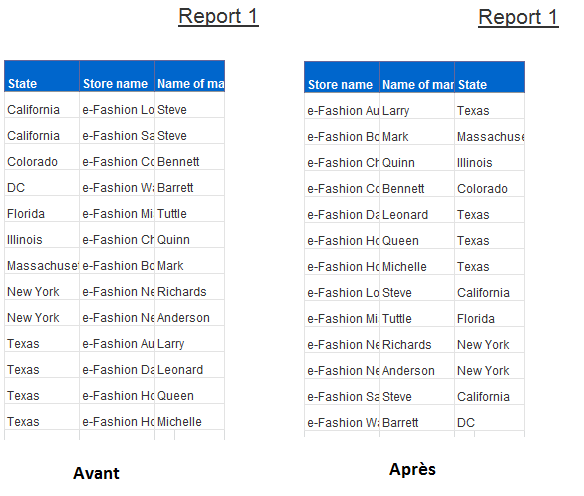
\includegraphics{images/dropcells.png}
  \caption{Allure du tableau avant et apr\`{e}s l'ex\'{e}cution du code}
	\label{figure:dropcells}
\end{figure}





